\documentclass[a4paper,twoside,12pt]{book}
%% === nezbytné balíčky:
\usepackage[T1]{fontenc}    % kódování písma
%\usepackage[IL2]{fontenc}  % kódování písma

\usepackage[utf8]{inputenc}     % vstupní znaková sada tohoto dokumentu: UTF-8
%\usepackage[cp1250]{inputenc}  % vstupní znaková sada tohoto dokumentu: Windows 1250
%\usepackage[latin2]{inputenc}  % vstupní znaková sada tohoto dokumentu: ISO Latin 2
\DeclareUnicodeCharacter{2029}{ }

\usepackage[czech]{babel} % česky psaná práce, typografická pravidla. Překládejte pomocí "latex.exe" nebo "pdflatex.exe"
%\usepackage{czech} % česky psaná práce. Překládejte pomocí "pdfCSlatex.exe" ("cslatex.exe" asi bude mít problém s balíkem geometry)

\usepackage[a4paper, hmarginratio=3:2]{geometry} % využití A4 stránky a nastavení okrajů (u vazby bude širší)

\usepackage{pdfpages} % pokud nemáte formulář "Zadání bak./dipl. práce" naskenovaný jako PDF, tak ZAKOMENTUJTE
\usepackage[hidelinks]{hyperref} % v PDF budou klikací odkazy ("hidelinks" je nebude rámovat)

%% === balíčky, které se mohou hodit:
%\usepackage{encxvlna} % postará se o spojky a předložky, které dle českých pravidel nesmí být na konci řádku. Dokumentace: http://texdoc.net/texmf-dist/doc/generic/encxvlna/encxvlna.pdf (chová se správně k "vnitřku" listings?)

\usepackage{graphicx} % balíček pro vkládání rastrových grafických souborů (PNG apod.)
%\usepackage{epsfig} % balíčky pro vkládání grafických souborů typu EPS
%\usepackage{float} % rozšířené možnosti umístění obrázků

%\usepackage{caption} % pro popisky obrázků, tabulek atd.

\usepackage{tabularx} % rozšířené možnosti tabulek
%\usepackage{tabu} % jiný balík pro rozšířené možnosti tabulek

\usepackage{listings}  % balíček vhodný pro ukázky zdrojového kódu v~textu práce/příloh. Nutno nastavit! http://ftp.cvut.cz/tex-archive/macros/latex/contrib/listings/listings.pdf
\usepackage{amsmath} % balíček pro pokročilou matematickou sazbu
%\usepackage{color} % pro možnost barevného textu
%\usepackage{fancybox} % umožňuje pokročilé rámečkování

%\usepackage{index} % nutno použít v případě tvorby rejstříku balíčkem makeindex
%\newindex{default}{idx}{ind}{Rejstřík} % zavádí rejstřík v případě použití balíku index
\usepackage{amssymb}
\usepackage[nice]{nicefrac}

\frenchspacing % za větou bude mezislovní mezera (v anglických textech je mezera za větou delší)
\widowpenalty=1000 % "síla" zákazu vdov (= jeden řádek ze začátku odstavce na konci stránky)
\clubpenalty=1000 % "síla" zákazu sirotků (= jeden řádek/slovo z konce odstavce samostatně na začátku stránky)
\brokenpenalty=1000 % "síla" zákazu zlomu stránky za řádkem, který má na konci rozdělené slovo

\topmargin=-15mm      % horní okraj trochu menší
\textwidth=150mm      % šířka textu na stránce
\textheight=240mm     % "výška" textu na stránce


\pagenumbering{arabic} % číslování stránek arabskými číslicemi
\pagestyle{plain}      % stránky číslované dole uprostřed

\parindent=0pt % odsazení 1. řádku odstavce
\parskip=7pt   % mezera mezi odstavci

\newcommand{\ti}{\textit} % zkrácený příkaz pro kurzívu
\newcommand{\tb}{\textbf} % zkrácený příkaz pro tučné písmo


%% --- zde jsou zavedeny některé "konstanty" - některé musíte změnit! --- %%
\newcommand{\cvut}{České vysoké učení technické v~Praze}
\newcommand{\fjfi}{Fakulta jaderná a fyzikálně inženýrská}
\newcommand{\ksi}{Katedra softwarového inženýrství}
\newcommand{\program}{Aplikace přírodních věd} % změňte, pokud máte jiný stud. program
\newcommand{\obor}{Aplikace softwarového inženýrství} % změňte, pokud máte jiný obor

\newcommand{\druh}{Výzkumný úkol} % nebo "Diplomová práce"
\newcommand{\woman}{} % pokud jste ŽENA, ZMĚŇTE na: ...{\woman}{a} (je to do Prohlášení)

\newcommand{\logoCVUT}{
\includegraphics{symbol_cvut_konturova_verze_cb.pdf}} % logo ČVUT -- podle grafického manuálu ČVUT platného od prosince 2016. Pokud nevyhovuje PDF-verze, tak použijte jinou variantu loga: https://www.cvut.cz/logo-a-graficky-manual -> "Symbol a logo ČVUT v Praze"). Pokud chcete logo úplně vynechat, zadejte místo "\includegraphics{...}" text "\vspace{35mm}"

% přesně podle formuláře "Zadání bak./dipl. práce" VYPLŇTE:
\newcommand{\nazevcz}{Webový systém pro testování znalostí studentů}    % český název práce (přesně podle zadání!)
\newcommand{\nazeven}{}          % anglický název práce (přesně podle zadání!)
\newcommand{\autor}{Bc. František Navrkal}   % vyplňte své jméno a příjmení (s akademickým titulem, máte-li jej)
\newcommand{\vedouci}{Ing. Martin Plajner} % vyplňte jméno a příjmení vedoucího práce, včetně titulů, např.: Doc. Ing. Ivo Malý, Ph.D.
\newcommand{\pracovisteVed}{Ústav teorie informace a automatizace, Akademie věd České republiky} % ZMĚŇTE, pokud vedoucí Vaší práce není z KSI
\newcommand{\konzultant}{--} % POKUD MÁTE určeného konzultanta, NAPIŠTE jeho jméno a příjmení
\newcommand{\pracovisteKonz}{--} % POKUD MÁTE konzultanta, NAPIŠTE jeho pracoviště

% podle skutečnosti VYPLŇTE:
\newcommand{\rok}{2017}  % rok odevzdání práce (jen rok odevzdání, nikoli celý akademický rok!)
\newcommand{\kde}{Praze} % studenti z Děčína ZMĚNÍ na: "Děčíně" (doplní se k "prohlášení")

% \newcommand{\klicova}{Klíčová slova}   % zde NAPIŠTE česky max. 5 klíčových slov
% \newcommand{\keyword}{Key words}       % zde NAPIŠTE anglicky max. 5 klíčových slov (přeložte z češtiny)
\newcommand{\abstrCZ}{Popis práce česky}    % zde NAPIŠTE abstrakt v češtině (cca 7 vět, min. 80 slov)
% \newcommand{\abstrEN}{Popis práce anglicky} % zde NAPIŠTE abstrakt v angličtině

\newcommand{\prohlaseni}{Prohlašuji, že jsem svůj výzkumný úkol vypracoval\woman{} samostatně a použil\woman{} jsem pouze podklady (literaturu, projekty, SW atd.) uvedené v přiloženém seznamu.} % text prohlášení můžete mírně upravit :-)

\newcommand{\podekovani}{Děkuji Ing. Martinu Plajnerovi za jeho pomoc a ochotu.} % NAPIŠTE poděkování, např. svému vedoucímu:
% Děkuji Ing. Eleonoře Krtečkové, Ph.D. za vedení mé bakalářské práce a za podnětné návrhy, které ji obohatily.
% NEBO:
% Děkuji vedoucímu práce doc. Pafnutijovi Snědldítětikaši, Ph.D. za neocenitelné rady a pomoc při tvorbě bakalářské práce.


\begin{document}
%%%%%%%%%%%% TITULNÍ STRANA -- na následujících cca 30 řádků NESAHEJTE!!!  Generuje se AUTOMATICKY %%%%%%%%%%%%
\thispagestyle{empty}

\begin{center}
	{\LARGE
		\cvut\par
		\fjfi
	}
    \vspace{10mm}

    \begin{tabular}{c}
		\tb{\ksi} \\[3pt]
		\tb{Obor: \obor}\\
    \end{tabular}

   \vspace{10mm} \logoCVUT \vspace{15mm}

   {\huge \tb{\nazevcz}\par}
   \vspace{5mm}
   {\huge \tb{\nazeven}\par}

   \vspace{15mm}
   {\Large \MakeUppercase{\druh}}

   \vfill
   {\large
    \begin{tabular}{ll}
    Vypracoval: & \autor\\
    Vedoucí práce: & \vedouci\\
    Rok: & \rok
    \end{tabular}
   }
\end{center}

\clearpage{\pagestyle{empty}\cleardoublepage} % prázdná stránka za tou "titulní", bez čísla

%%%%%%%%%%%% ZADÁNÍ PRÁCE %%%%%%%%%%%%
% Zadání (podepsané děkanem!) musíte NASKENOVAT. Ideálně jako 2stránkové PDF (soubor "zadani_cele.pdf").
% Před svázáním to v jednom výtisku VYMĚNÍTE ZA ORIGINÁLNÍ ZADÁNÍ (podepsané děkanem fakulty)!
\newpage  % SEM NESAHEJTE!
\thispagestyle{empty} % SEM NESAHEJTE!

%% zde podle toho, jak jste zadání naskenovali, VYBERTE variantu A, B nebo C:
%
% --- varianta A: zadání naskenované jako 2stránkové PDF:
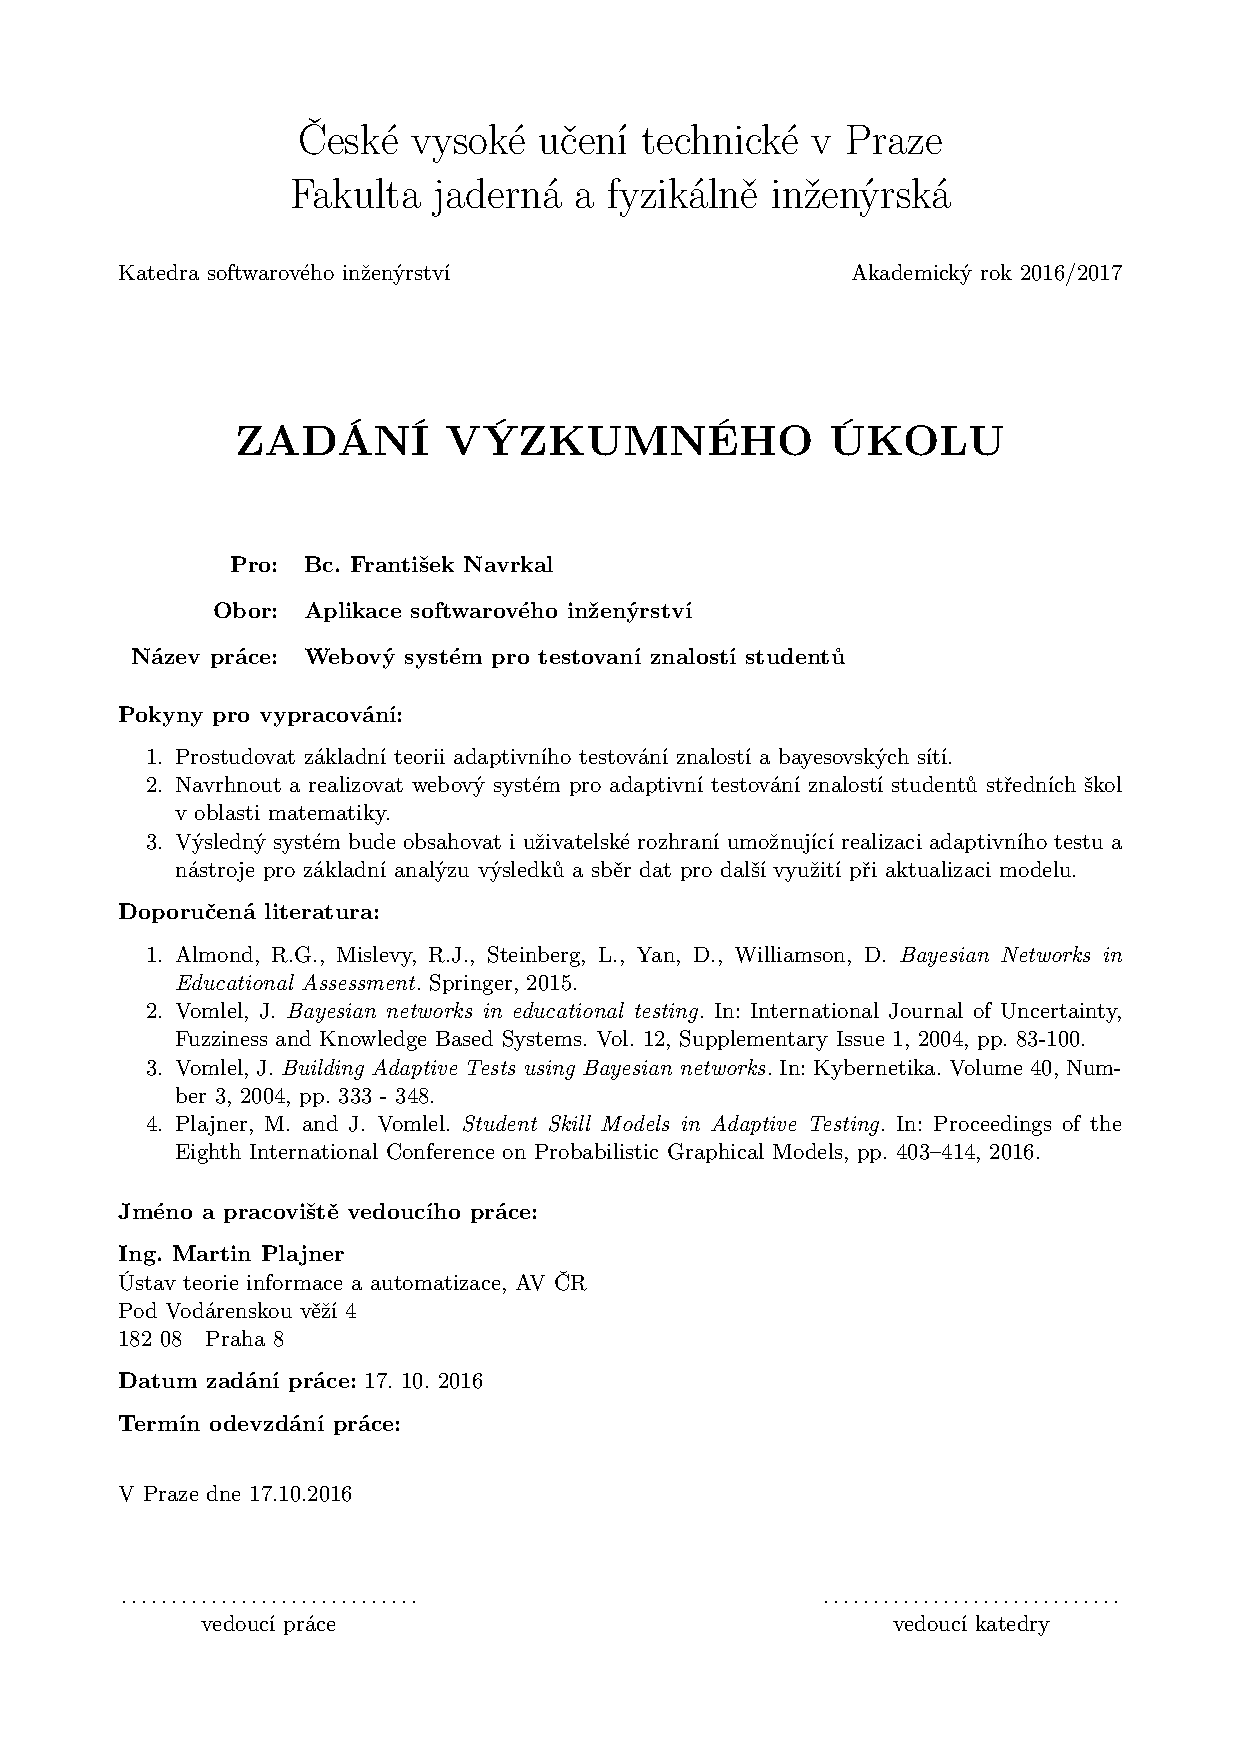
\includepdf{zadani_cele.pdf} % NAHRAĎTE správným souborem!
%
%% --- varianta B: zadání naskenované jako jednotlivé stránky:
%\includepdf[pages={1}]{zadani1.pdf} % 1. strana zadání v PDF
%\includepdf[pages={1}]{zadani2.pdf} % 2. strana zadání v PDF
%
%% --- varianta C: zadání naskenované jako 2 samostatné obrázky:
%% 1. strana zadání
%\begin{center}
%     \includegraphics[width=1\textwidth]{zadani1.jpg}
%\end{center}
%% 2. strana zadání
%\newpage  % SEM NESAHEJTE!
%\thispagestyle{empty} % SEM NESAHEJTE!
%\begin{center}
%     \includegraphics[width=1\textwidth]{zadani2.jpg}
%\end{center}


%%%%%%%%%%%% Prohlášení -- SEM NESAHEJTE! Generuje se automaticky z výše nastavených maker \kde{} a \prohlaseni{}. %%%%%%%%%%%%
\newpage % SEM NESAHEJTE!
\thispagestyle{empty}  % SEM NESAHEJTE!

~ % SEM NESAHEJTE!
\vfill % prázdné místo. SEM NESAHEJTE!

\tb{Prohlášení} % SEM NESAHEJTE!

\vspace{1em} % vertikální mezera. SEM NESAHEJTE!
\prohlaseni

\vspace{2em}  % SEM NESAHEJTE!
\hspace{-0.5em}\begin{tabularx}{\textwidth}{X c}  % SEM NESAHEJTE!
V \kde\ dne .................... &........................................ \\	% SEM NESAHEJTE!
	& \autor
\end{tabularx}	% SEM NESAHEJTE!


%%%%%%%%%%%% Poděkování  %%%%%%%%%%%%
\newpage
\thispagestyle{empty}

~
\vfill % prázdné místo


% -- následující kus kódu (do "%%%%%%%%%%%% ABSTRAKT") můžete odstranit, pokud nechcete psát poděkování:
\tb{Poděkování}

\vspace{1em} % vertikální mezera
\podekovani
\begin{flushright}
\autor
\end{flushright}  % <------- tady končí stránka s poděkováním


%%%%%%%%%%%% ABSTRAKT atp. Je generován AUTOMATICKY podle maker nastavených na začátku souboru) %%%%%%%%%%%%
% \newpage   % SEM NESAHEJTE!
% \thispagestyle{empty}   % SEM NESAHEJTE!
%
% % příprava:    (na následujících 8 řádků NESAHEJTE!)
% \newbox\odstavecbox
% \newlength\vyskaodstavce
% \newcommand\odstavec[2]{%
%     \setbox\odstavecbox=\hbox{%
%          \parbox[t]{#1}{#2\vrule width 0pt depth 4pt}}%
%     \global\vyskaodstavce=\dp\odstavecbox
%     \box\odstavecbox}
% \newcommand{\delka}{120mm} % šířka textů ve 2. sloupci tabulky
%
% % použití přípravy:    % dovnitř "tabular" vůbec NESAHEJTE!
% \begin{tabular}{ll}
%   {\em Název práce:} & ~ \\
%   \multicolumn{2}{l}{\odstavec{\textwidth}{\bf \nazevcz}} \\[1em]
%   {\em Autor:} & \autor \\[1em]
%   {\em Studijní program:} & \program \\
%   {\em Obor:} & \obor \\
%   {\em Druh práce:} & \druh \\[1em]
%   {\em Vedoucí práce:} & \odstavec{\delka}{\vedouci\\ \pracovisteVed} \\
%   {\em Konzultant:} & -- %\odstavec{\delka}{\konzultant \\ \pracovisteKonz}  % VYMAŽTE text "-- %" v případě, že jste neměli konzultanta
%  \\[1em]
%   \multicolumn{2}{l}{\odstavec{\textwidth}{{\em Abstrakt:} ~ \abstrCZ  }} \\[1em]
%   {\em Klíčová slova:} & \odstavec{\delka}{\klicova} \\[2em]
%
%   {\em Title:} & ~\\
%   \multicolumn{2}{l}{\odstavec{\textwidth}{\bf \nazeven}}\\[1em]
%   {\em Author:} & \autor \\[1em]
%   \multicolumn{2}{l}{\odstavec{\textwidth}{{\em Abstract:} ~ \abstrEN  }} \\[1em]
%   {\em Key words:} & \odstavec{\delka}{\keyword}
% \end{tabular}



%%%%%%%%%%%% Obsah práce ... je generován AUTOMATICKY %%%%%%%%%%%%
\newpage  % SEM NESAHEJTE!
\parskip=0pt
\tableofcontents % SEM NESAHEJTE!
\parskip=7pt
\newpage % SEM NESAHEJTE!


%--------------------------------------------------------
%|         Zde začíná SAMOTNÁ PRÁCE (text)              |
%--------------------------------------------------------

\chapter*{Úvod} % SEM NESAHEJTE!
\addcontentsline{toc}{chapter}{Úvod} % SEM NESAHEJTE!
%
Zde napište text úvodu (1-3 strany, nerozdělujte na podkapitoly) nebo jej vložte ze samostatného souboru: např. příkazem \texttt{\textbackslash input\{vnitrek\_uvod.tex\}}.
%
%\input{vnitrek_uvod.tex}

%---------------------------------------

\chapter{Adaptivní testování obecně}
Adaptivní počítačové testování je způsob získávání informací o znalostech studenta, při kterém se průběh testování mění na základě informací získaných v jeho průběhu (nebo i před jeho zahájením). V anglicky psané literatuře se pro toto používá označení computerized adaptive testing (CAT). Využití CAT umožňuje kombinovat výhody individuálního testování jako zvýšená přesnost a úspora času i námahy testovaného s možností hromadného testování.

\section{Motivace}
Hromadně aplikovaný test musí, aby fungoval dobře pro širokou škálu úrovní jednotlivých měřených dovedností, obsahovat otázky různé obtížnosti. Pokud by na příklad neobsahoval lehké otázky, nemohl by test přesně měřit nízkou úroveň příslušných dovedností.

Tento fakt ovšem znamená, že zdatný student ve statickém testu musí nejdříve odpovědět na mnoho pro něj jednoduchých otázek, než se dostane k otázkám, které mají nějakou vypovídací hodnotu o jeho dovednostech. Toto vede k mrhání času a námahy studenta, přináší to též do procesu testování nechtěné faktory jako chyby z nedbalosti způsobené nudou.

V případě, že je úroveň měřených dovedností studenta naopak nízká, hrozí zase zmatek, frustrace a nekvalitní data, pokud slabý student správnou odpověď jen náhodou uhodne. \cite[strana 10]{Wainer2000}


\section{Průběh adaptivního testování}

Samotný průběh adaptivního testování sestává z opakování těchto kroků:
\begin{enumerate}
	\item Výběr otázky na základě modelu znalostí studenta dle nějakého výběrového kritéria.
	\item Zobrazení otázky studentovi, získání odpovědi a její vyhodnocení.
	\item Vložení získaných informací do modelu znalostí studenta a jeho aktualizace.
	\item Kontrola ukončovacích kritérií a případné ukončení testu při jejich dosažení.
\end{enumerate}

Tomuto ovšem musí předcházet tvorba celého testu a příslušného modelu znalostí. Po proběhnutí mnoha případů testování lze na základě analýzy informací získaných o jejich průběhu model vylepšit.

% -------------------------------------------------
\chapter{Znalostní model (Bayesovské sítě)}
Pro výběr otázek v rámci našeho přístupu k adaptivnímu testování se používá bayesovských sítí. Jedná se o grafický model (ve smyslu teorie grafů) popisující vztahy mezi náhodnými veličinami pomocí podmíněných pravděpodobnostních rozdělení.

\section{Formální definice}
Bayesovskou síť pro naše účely můžeme definovat formálně jako uspořádanou dvojici orientovaného acyklického grafu $B_S = (V,E)$ (tzv. struktura sítě), kde každému prvku $i \in V$ odpovídá náhodná veličina $X_i$, a množiny $B_P$  funkcí $P(X_i\,|\,(X_j)_{j\in pa(i)})$, které udávají podmíněné pravděpodobnostní rozdělení $X_i$ v závislosti na hodnotě proměnných odpovídajících (přímým) předchůdcům $i$ v $B_S$ značeným jako $pa(i)$. Množinu všech náhodných veličin budu značit $X=\{X_i\,|\,i \in V\}$.

V našem případě budou $X_i$ nabývat jen určitých diskrétních hodnot z množin $\mathbb{X}_i$, takže si prvky $B_P$ můžeme také představovat prostě jako funkce zobrazující vektor stavů předchůdců $i$ v $B_S$ na vektor pravděpodobností stavů $X_i$. Prakticky lze takového funkce zapsat jako tak zvanou tabulku podmíněných pravděpodobností.

\section{Neformální popis}
Bayesovské sítě vlastně popisují statisticky získané a popsané kauzální vztahy mezi nějakými pozorovanými událostmi. V našem případě půjde kauzální vztah mezi odpověďmi studenta na otázky v testu a jeho měřenými dovednostmi.

Jeden z předpokladů pro běžné výpočty v bayesovských sítích je, že pro každou veličinu $X_i$ platí, že je podmíněně nezávislá na veličinách, které  \textbf{ne}jsou reprezentovány jejími potomky v síti, podmíněno znalostí stavu veličin reprezentovaných jejími předky v síti. Zkráceně: každá veličina je podmíněně nezávislá na svých nepotomcích podmíněno znalostí svých předků.

Tento požadavek v praxi nelze striktně splnit, protože by model musel pokrýt opravdu všechny předpoklady pro správné zodpovězení otázek. Modely se tedy snaží pokrýt jen ty nejvíce relevantní a nejlépe měřitelné. Komplexita zamšlených modelů také značně zvyšuje nároky na sběr dat pro jejich návrh.

Pro výpočty na bayesovské síti je také zpravidla nutné mít k dispozici nějaká apriorní pravděpodobnostní rozdělení $X_i$, a to aspoň u těch proměnných, jejichž uzly v síti nemají předky.

\section{Příklady}
\label{sec:net_examples}
V \cite{almond_tlustospis} je hned v úvodu jako příklad uvedena síť na obrázku \ref{fig:almond_BN_example}. Uzly s kroužky udávají jednotlivé dovednosti (čtení, psaní, poslech, mluvení) a uzly s trojúhelníky udávají stavy vyhodnocení úkolů vyžadujících jednotlivé kombinace těchto dovedností.

\begin{figure}
  \centering
    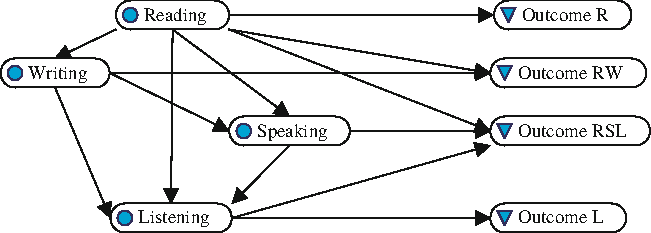
\includegraphics[width=0.8\textwidth]{almond_BN_example.pdf}
  \caption{Příklad bayesovské síťě z \cite{almond_tlustospis}.}
  \label{fig:almond_BN_example}
\end{figure}

Pro představu o topologii sítí, které ve svém výzkumu používal vedoucí práce, lze také použít přímo jednu z nich. Na obrázku \ref{fig:plajner16} zelené uzly reprezentují jednotlivé dovednosti a žluté uzly otázky. Uzel \emph{S8} (celková dovednost, konkrétně znalost jednoduchých funkcí) je předchůdcem všech uzlů, následují ostatní zelené uzly (jednotlivé prvky celkové dovednosti: znalost polynomů, exponenciálních funkcí a tak dále) a na konec žluté uzly, které reprezentují jednotlivé úlohy v testu.

\begin{figure}
  \centering
    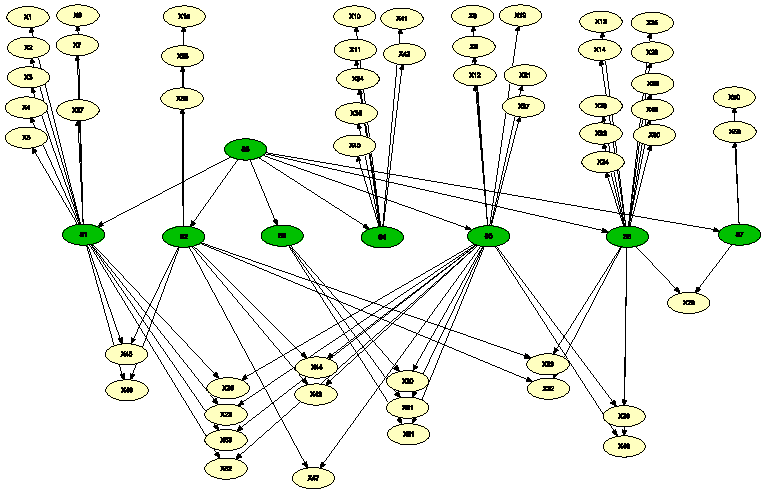
\includegraphics[width=0.85\textwidth]{complex_BN_plajner16.pdf}
  \caption{Příklad bayesovské síťě z \cite{plajner16}.}
  \label{fig:plajner16}
\end{figure}

\section{Dovednosti a otázky}
Množina všech náhodných veličin $X$ se ve zde blíže probíraných případech bude typicky dělit na 2 disjunktní podmnožiny $S \cup Q = X$, kde $S$ je množina veličin představujících dovednosti a $Q$ otázky (je tomu tak v obou zmíněných příkladech a předpkládám to i ve své webové aplikaci). Dále ještě mohou být v bayesovské síti zastoupeny jako náhodné veličiny další informace o studentovi jako třeba věk, pohlaví nebo výsledky jiného testování.

Vyhodnocení adaptivního testu bude znamenat na základě získaných dat vypočítat pravděpodobnostní rozdělení veličin z $S$.

\section{Aktualizace modelu v průběhu testování}
Informace získané v průběhu testování se do modelu vkládají tak, že se apriorní rozdělení veličiny z $Q$ nahradí formálně rozdělením, kde je jeden ze stavů již jistý (tedy vektor pravděpodobnostní stavů je pak vektor obsahující jeden prvek s hodnotou 1 a všechny ostatní s hodnotou 0). Toto umožní aktualizaci rozdělení ostatních veličin jak z $S$, tak z $Q$, jejichž stav není v daném okamžiku ještě známý.


% --------------------------------------

\chapter{Návrh adaptivního testu}
Možností, jak navrhnout test je nespočet. Pro představu krátce shrnu jako příklad článek podrobně popisující návrhu testu, konrétně \cite{vomlel_plajner2015}.

\section{Návrh obsahu a sběr dat}
Nejdříve autoři navrhli statický test, ten předložili malé skupině studentů. Na základě zpětné vazby pak vytvořili další, pro studenty srozumitelnšjší, návrh, ze kterého byly také odebrány otázky, které se ukázaly neefektivní pro zisk informací.

Test nakonec obsahoval 29 úloh, které se dále rozdělily celkem na 53 podúloh. Úlohy byly alternativně vyhodnocovány pomocí bodového ohodnocení, nebo prostě jen jako správně či špatně vypracované.

Sběru dat se celkem zúčastnilo 281 studentů. O těchto studentech si autoři sesbírali také některá jejich osobní data jako věk, pohlaví, jméno a jejich známky z matematiky, chemie a fyziky za poslední 3 ročníky.


\section{Srovnání znalostních modelů}
V článku autoři porovnaly celkem 14 různých modelů, které se lišily mj. počtem uvažovaných stavů náhodných veličin, počtem měřených dovedností a zahrnutím osobních dat studentů.

Struktura sítě byla vždy pro daný srovnávaný model pevná a tabulky podmínených pravděpodobností se vždy v rámci desetinásobné křížové validace odhadly (naučily) na základě $\nicefrac{9}{10}$ náhodně vybraných případů (učící množiny). Jednotlivé modely pak byly porovnávány na základě chování modelu v simulacích na zbývající $\nicefrac{1}{10}$ případů (testovací množinu).

Modely autoři konkrétně porovnávaly na základě míry úspěšnosti odhadu hodnocení zatím v simulaci neřešených úloh na základě úloh již v dané simulaci vyřešených a vyhodnocených, to celé v závislosti na počtu vyřešených úloh (počtu odsimulovaných kroků testování).

Jako kritérium výběru úlohy v simulacích autoři použili maximalizaci očekávaného informačního zisku (neboli poklesu entropie) stavu dovedností po vyhodnocení kandidátní úlohy.

\section{Závěr}
Autoři došli k tomu, že příliš jednoduché modely si nevedly dobře -- ukázalo se jako výhodné uvažovat raději 3 než pouze 2 stavy u dovednostních veličin.

Zahrnutí osobních údajů o studentovi do modelu vylepšilo úspěšnost předpovědí jen v počátečních krocích testování, poté měly pouze malý pozitivní, nebo dokonce negativní efekt.

Složitější z modelů pravděpodobně postihl tak zvaný over-fitting, to jest naučené tabulky podmíněných pravděpodobností nezobecňovaly dobře vztahy z učící množiny pro testovací množinu, takže si nakonec nevedly dobře.

V jejich novějším článku \cite{plajner16} používají autoři mj. síť na obrázku \ref{fig:plajner16}, která se liší od té z \cite{vomlel_plajner2015} hlavně přidáním souhrné dovednostní veličiny jako předchůdce všech ostatních veličin. Tato síť měla hlavně ve spojení s jejich novým algoritmem pro učení z testovací množiny mnohem lepší úspěšnost předpovědí.

% TODO: link comparison chart figure form plajner16



\chapter*{Závěr} % SEM NESAHEJTE!
\addcontentsline{toc}{chapter}{Závěr} % SEM NESAHEJTE!
%
Zde napište text úvodu (1-3 strany, nerozdělujte na podkapitoly) nebo jej vložte ze samostatného souboru: např. příkazem \texttt{\textbackslash input\{vnitrek\_zaver.tex\}}.
%
%\input{vnitrek_zaver.tex}


%%%%%%%%%%%% SEZNAM POUŽITÝCH ZDROJŮ (LITERATURA) %%%%%%%%%%%%
\clearpage  % SEM NESAHEJTE!
\addcontentsline{toc}{chapter}{Literatura} % SEM NESAHEJTE!

\begin{thebibliography}{99}
	% formát: ČSN ISO 690. Můžete si to vygenerovat na http://www.citacepro.com (přihlaste se přes odkaz "ČVUT"), umí to vygenerovat TeX
	% řazení: abecedně podle autora (resp. prvního slova, není-li znám autor)
	\bibitem{almond_tlustospis} Almond, R.G., Mislevy, R.J., Steinberg, L., Yan, D., Williamson, D. \textit{Bayesian Networks in Educational Assessment.} Springer, 2015.
	\bibitem{vomlel_obec} Vomlel, J. \textit{Bayesian networks in educational testing.} International Journal of Uncertainty, Fuzziness and Knowledge Based Systems. Vol. 12, Supplementary Issue 1, 2004, pp. 83-100.
  \bibitem{vomlel_building} Vomlel, J. \textit{Building Adaptive Tests using Bayesian networks.} Kybernetika. Volume 40, Number 3, 2004, pp. 333 - 348.
	\bibitem{plajner16} Plajner, M., J. Vomlel. \textit{Student Skill Models in Adaptive Testing.} Proceedings of the Eighth International Conference on Probabilistic Graphical Models, pp. 403–414, 2016.

	\bibitem{Wainer2000} WAINER, Howard. a Neil J. DORANS. \textit{Computerized adaptive testing: a primer}. 2nd ed. Mahwah, N.J.: Lawrence Erlbaum Associates, 2000. ISBN 08-058-3511-3.
	\bibitem{vomlel_plajner2015} Plajner, M., J. Vomlel. \textit{Bayesian network models for adaptive testing.} Proceedings of the Twelfth UAI Conference on Bayesian Modeling Applications Workshop-Volume 1565. CEUR-WS. org, 2015. p. 24-33.
\end{thebibliography}


%%%%%%%%%%%% PŘÍLOHY PRÁCE %%%%%%%%%%%%
\newpage % SEM NESAHEJTE!
\addcontentsline{toc}{chapter}{Přílohy} % SEM NESAHEJTE!
\appendix % SEM NESAHEJTE!


%%%%%%%%%%%% Příloha A (tj. 1. kapitola v rámci příloh) %%%%%%%%%%%%

\chapter{Název první přílohy}
%
Zde napište text první přílohy nebo jej vložte, např.: \texttt{\textbackslash input\{priloha\_A.tex\}}.
%
%\input{priloha_A.tex} % text vkládán ze souboru, kde je i příkaz \chapter{...}


\end{document} % SEM NESAHEJTE! Konec.
